\newpage
\section{Einleitung}
Hexiwear ist eine von Mikroelektronika entwickelte Sensor Platform mit OLED-Display, umfangreichen Softwarefunktionen und vielen weiteren Komponenten. Die Hard- sowie Software rund um die Hexiwear wird im Umfang dieses Projektes erweitert, damit sie als universeller Sensor- und Aktorknoten für zukünftige Projekte verwendet werden kann. Weiter wird zu Demonstrationszwecken eine Hausautomations Steuerung mit der Software openHAB auf einem Raspberry Pi eingerichtet und mit der Hexiwear verknüpft. Abb. \ref{fig:komp_abstrakt} bietet eine Übersicht über die verwendeten Komponenten und deren Beschaltung.

\begin{figure}[H]
	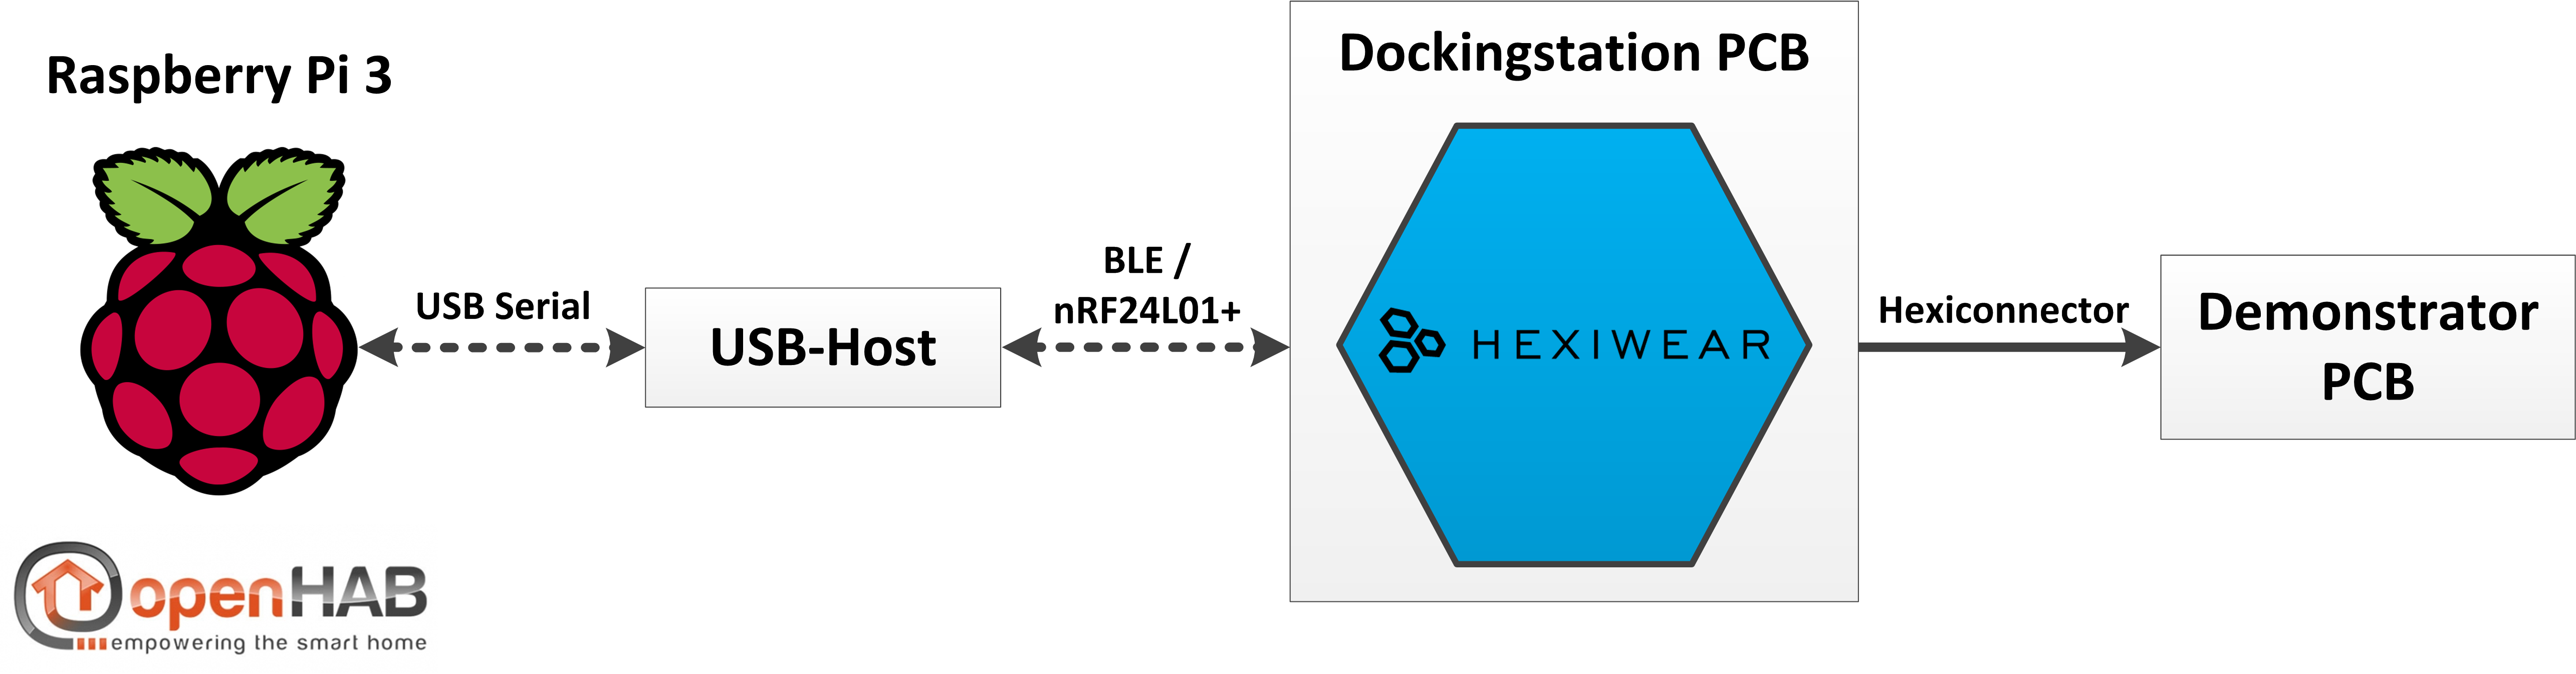
\includegraphics[width=1\textwidth]{Illustrationen/1-Einleitung/Komponentenuebersicht_grob.png}
	\caption{abstrahiertes Blockschaltbild}
	\label{fig:komp_abstrakt}
\end{figure}

Der Projektablauf kann grob in vier Teile mit entsprechenden Arbeitspaketen gegliedert werden. In Abb. \ref{fig:projektplan} ist der Projektplan in Form eines Ablaufdiagramms gemäss den vier Teilen: Initialphase, PCB, Hexiwear und Raspberry Pi / openHAB dargestellt. Der detaillierte Projektplan kann im Anhang nachgeschlagen werden.

\begin{figure}[H]
	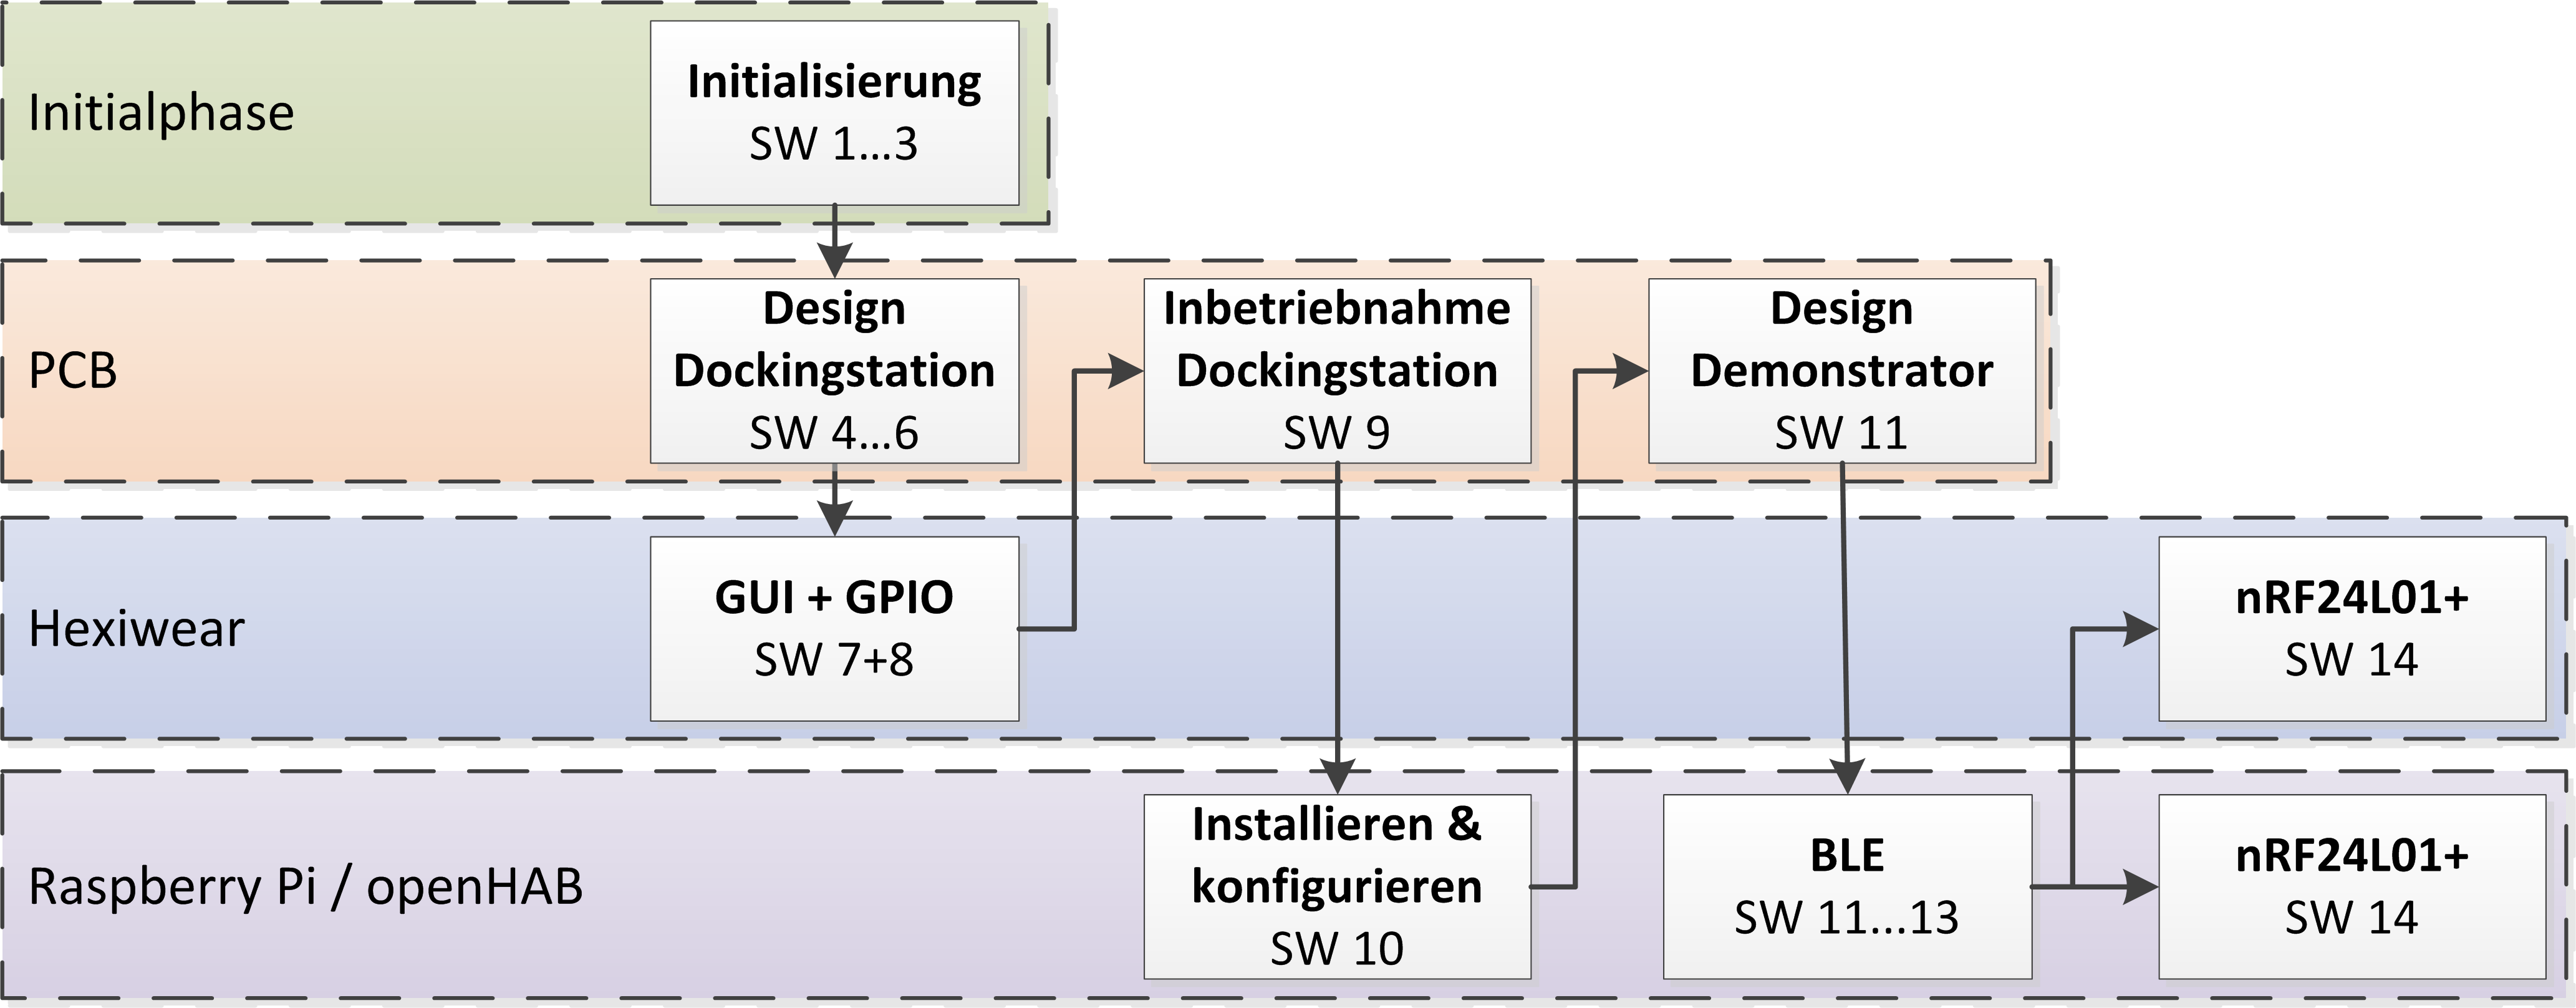
\includegraphics[width=1\textwidth]{Illustrationen/1-Einleitung/Zeitplan.png}
	\caption{Projektplan Ablaufdiagramm}
	\label{fig:projektplan}
\end{figure}

Die verschiedenen Arbeitspakete werden im folgenden Abschnitt kurz erläutert:
\begin{itemize}
	\item \textbf{Initialisierung:} Der Anfang des Projekts gestaltete sich durch einlesen in die Aufgabenstellung sowie einer Technologierecherche über die zu verwendende Hard- und Software. Weiter wurden die Dokumente zur Projektplanung und Dokumentation aufgesetzt. Da die Projektdokumentation in Latex verfasst wurde, war ein entsprechendes Selbststudium nötig. Zum Schluss der Initialphase wurde das Pflichtenheft ausgearbeitet und dem Dozenten vorgelegt.
	
	\item \textbf{Design Dockingstation:} Dieses Arbeitspaket umfasst das Zeichen des Schemas, evaluieren der Komponenten sowie das Layouten der Schaltung. Nach Abschluss des Designs wurde das PCB als Prototyp zur Fertigung an der HSLU aufgegeben. Die durch den Fertigungsprozess entstandene Wartezeit wurde mit dem nächsten Arbeitspaket überbrückt.
	
	\item \textbf{GUI + GPIO:} Zur Halbzeit des Semesters wurde die Software der Hexiwear erweitert. Dabei wurde ein neuer GUI Screen designt und eingebunden. Dieser wurde mit zwei Funktionbuttons zur Ansteuerung von LEDs versehen.
	
	\item \textbf{Inbetriebnahme Dockinstation:} Das PCB wurde bestückt und in Betrieb genommen. Sämtliche Funktionen des PCBs wurden dabei getestet.
	
	\item \textbf{Installation \& Konfiguration:} Die Software openHAB wurde auf dem Raspberry installiert und konfiguriert. Dabei wurde bereits eine Sitemap eingerichtet mit der die Hexiwear später verknüpft werden soll.
	
	\item \textbf{Design Demonstrator:} Um die Funktion der Smart-Home Applikation präsentieren zu können wurde die Schaltung für ein Demonstrator PCB designt, das Layout erstellt und das PCB zur Fertigung in Auftrag gegeben. Nach der Fertigung konnte das PCB bestückt und getestet werden.
	
	\item \textbf{BLE:} Das Arbeitspaket BLE stellte sich als sehr Zeitintensiv heraus. Zum Thema musste viel recherchiert und ausprobiert werden. Desshalb wurde das Arbeitspaket nach drei Wochen abgebrochen und eine Ist-Aufnahme durchgeführt.
	
	\item \textbf{nRF24L01+:} Zum Schluss wurde der alternative drahtlos Kommunikationspfad nRF24L01+ mit tatkräftiger Unterstützung des Dozenten auf der Hexiwear und dem Raspberry Pi implementiert. Dabei wurde auf dem Raspberry das Mikrocontrollerboard USB-Host über USB angeschlossen. Dieses Arbeitspaket konnte ebenfalls Mangels Zeit nicht Fertiggestellt werden.
\end{itemize}